\documentclass[a4paper,11pt]{article}

% ---------- Packages ----------
\usepackage[margin=2.5cm]{geometry}
\usepackage{amsmath, amssymb, amsthm, mathtools}
\usepackage{algorithm}
\usepackage{algpseudocode}
\usepackage{enumitem}
\usepackage{graphicx}
\usepackage{booktabs}
\usepackage{hyperref}
\usepackage{xcolor}

\usepackage{tikz}
\usetikzlibrary{automata,positioning,arrows.meta}

% ---------- Theorem Environments ----------
\newtheorem{theorem}{Theorem}
\newtheorem{lemma}{Lemma}
\newtheorem{definition}{Definition}
\newtheorem{proposition}{Proposition}
\newtheorem{corollary}{Corollary}

% ---------- Custom Commands ----------
\newcommand{\R}{\mathbb{R}}
\newcommand{\N}{\mathbb{N}}
\newcommand{\Z}{\mathbb{Z}}
\newcommand{\Alphabet}{\Sigma}
\newcommand{\eps}{\varepsilon}
\newcommand{\set}[1]{\left\{ #1 \right\}}
\newcommand{\abs}[1]{\left| #1 \right|}
\newcommand{\ceil}[1]{\left\lceil #1 \right\rceil}
\newcommand{\floor}[1]{\left\lfloor #1 \right\rfloor}

% ---------- Section Style ----------
\renewcommand{\thesubsection}{(\alph{subsection})}
\renewcommand{\thesection}{}

% ---------- Algorithm Style ----------
\algrenewcommand\algorithmicrequire{\textbf{Input:}}
\algrenewcommand\algorithmicensure{\textbf{Output:}}

% ---------- Title Info ----------
\title{\textbf{CSE2315 --- Assignment 8}}
\author{Vlad Paun \\ 6152937}
\date{\today}

% ---------- Document ----------
\begin{document}

	\maketitle

	\section{Exercise 1}
	Consider the problem Hamiltonian Circuit (HAMC):
	\[
	\set{(V,E) \mid \text{The graph } G=(V,E) \text{ contains a simple cycle } \pi \text{ such that } \forall v \in V : v \in \pi}
	\]

	In a different notation we would write:\\
	\textbf{Name:} Hamiltonian Circuit (HAMC)\\
	\textbf{Input:} A graph $G=(V,E)$.\\
	\textbf{Question:} Is there a simple cycle $\pi$ in $G$ such that all vertices $v \in V$ are in that cycle?

	Now take the following reduction from HAMC to HAMP, given an instance $G=(V,E)$ of HAMC:
	\begin{enumerate}[label=\Roman*.]
		\item Copy $G$ and add 2 new nodes $a,b$ to $V$.
		\item Pick some vertex $v_x \in V$: connect $b$ to all neighbours of $v_x$ and connect $a$ to $v_x$.
	\end{enumerate}

	Show that this reduction is not reliable.

	\textit{Note: this can be quite challenging! Try and apply the reduction on some graphs and see what happens first, get a feeling for how the reduction influences the graphs.}

	\textbf{Answer: }The reduction is not reliable because the following does not hold: $\langle G \rangle\notin HAMC \to f(\langle G\rangle)\notin HAMP$. Take as a counterexample the graph $G=(\set{v_1,v_2,v_3},\set{\set{v_1,v_2},\set{v_2,v_3}})$. This graph does not have a Hamiltonian Circuit. However, if we take $f(\langle G\rangle)$ and let the $v_x$ that is picked in step II be $v_2$, then we obtain the new graph: $$G'=(\set{v_1,v_2,v_3,a,b},\set{\set{v_1,v_2},\set{v_2,v_3},\set{v_1,b},\set{v_3,b},\set{v_2,a}})$$which has a Hamiltonian path $(a,v_2,v_3,b,v_1)$

	\section{Exercise 2}
	After many hours of hard work, Prof. P. E. Kwalsenpee has managed to create an algorithm TSP-Decider that can solve the decision variant of TSP in polynomial time. That is, given a set
	\[
	S=\set{s_i}_{i=1}^n
	\]
	of cities, a $n \times n$ intercity distance matrix $D=[d_{i,j}]$ where $d_{i,j}\in \mathbb{Z}^+$ and a positive integer $k$, the algorithm will accept if and only if there is a tour through all vertices in $S$ such that the total cost of the tour is $\leq k$.

	\subsection{Explain how we can also use TSP-Decider to decide the Hamiltonian Circuit problem in polynomial time.}

	We define a reduction $HAMC \leq_P TSP$ by using the following mapping function $f$:
	\begin{align*}
		&f:\Alphabet^*\to\Alphabet^*\\
		&f(\langle G=\set{V,E}\rangle) = \langle S,D,k\rangle
	\end{align*}
	Where $S=V$,$k=|V|$ and $D=[d_{i,j}]$ where $d_{i,j}=1$ if $\set{v_i,v_j}\in E$ or $\infty$ otherwise.
	$f$ defines a valid Karp reduction as it is both efficient (computable in polynomial time) and reliable.
	\begin{enumerate}
		\item \textbf{Efficiency: }The function $f$ needs to write 3 things on the tape: $S$,$D$ and $k$:
		\begin{itemize}
			\item S is just a copy of $V$ of the original graph, so it can be written in linear time
			\item The matrix $D$ is $|V|\times |V|$, so the size is polynomial in the size of the input. And actually calculating each cell of the matrix is still polynomial, as you just need to look it up in $E$, so it would be $O(|E|)$. Overall creating D would be $O(|E|\cdot|V|^2)$
			\item $k$ is just $|V|$, so you just need to go through all the nodes, which is linear.
		\end{itemize}
		Therefore, overall the function $f$ is computable in polynomial time.
		\item \textbf{Reliability: } We need to prove $\langle G \rangle\in HAMC \iff f(\langle G\rangle)\in TSP$:
		\begin{itemize}
			\item $\langle G \rangle\in HAMC \to f(\langle G\rangle)\in TSP$: $G$ has a Hamiltonian cycle, so there is a simple cycle that goes through all the nodes. The edges of this cycle have weight exactly $1$ in our $TSP$ instance, and this cycle has exactly $|V|=k$ edges. Therefore, in our $TSP$ instance, there is a tour containing $k$ edges of weight 1, so a tour of overall weight $k$.
			\item $f(\langle G\rangle)\in TSP\to \langle G \rangle\in HAMC $: The constructed $TSP$ instance has a tour going through all vertices of length at most $k=|V|$. Such a tour must also have exactly $|V|$ edges. This means that, by our construction, where edges have length either $1$ or $\infty$, all the edges of the tour have length $1$. These are exactly the edges of the graph $G$. So the tour only uses edges from $E$, so it corresponds to a Hamiltonian cycle in $G$.
		\end{itemize}
	\end{enumerate}

	\subsection{Given this decision algorithm by the professor and an instance $(S,D,k)$ of TSP, give a polynomial time algorithm that returns an actual TSP-tour through the cities with total cost of at most $k$, if such a tour exists. If not, the algorithm should return \texttt{nil}.}
	\textsc{Find-TSP-Tour($S,D,k$)}
	\begin{enumerate}
		\item Run \textsc{TSP-Decider($S,D,k$)}
		\begin{itemize}
			\item if it rejects, return \texttt{nil}
		\end{itemize}
		\item For every unordered pair of distinct vertices $(v_i,v_j)$:
		\begin{itemize}
			\item Set $d_{i,j}=d_{j,i}=k+1$ temporarily
			\item Run \textsc{TSP-Decider($S,D,k$)}
			\item if it accepts keep the change
			\item if it rejects, revert to the old $d$ values
		\end{itemize}
		\item After all pairs useless edges have been processed, the set of edges left with weights under $k$ should encode the tour.
	\end{enumerate}

	\section{Exercise 3}
	An important problem in analysing social networks is the question whether there are persons in the network who occur in more than one large clique of the network. Therefore, we consider the following problem:\\
	\textbf{Name} Important Node\\
	\textbf{Instance} an undirected graph $G=(V,E)$, and two positive integers $K>1$ and $L>1$.\\
	\textbf{Question} do there exist at least $K$ nodes $v \in V$ such that $v$ occurs in at least two different cliques of $G$, each containing at least $L$ nodes?\\

	Show that Important Node is an NP problem.\\
	\textbf{Answer: }The following represents a polynomial time verifier for the problem, where the certificate $c$ encodes:
	\begin{itemize}
		\item the $K$ important nodes
		\item for each of those nodes, two cliques of size at least $L$ that both contain the node
	\end{itemize}

	\begin{quote}
		$V=$ "On input $\langle G,K,L, c\rangle$, where
		\[
		c=\big((v_1,C_{1,1},C_{1,2}),\dots,(v_K,C_{K,1},C_{K,2})\big),
		\]
		do the following:
		\begin{enumerate}
			\item Check that the certificate contains at least $K$ triples, all with distinct nodes.
			\item For each $i\in\set{1,\dots,K}$:
			\begin{enumerate}
				\item Check that $v_i\in V$
				\item Check that $|C_{i,1}|\geq L$ and $|C_{i,2}|\geq L$.
				\item Check that $C_{i,1}$ and $C_{i,2}$ are both valid cliques.
			\end{enumerate}
			\item If all checks succeed, accept, otherwise reject."
		\end{enumerate}
	\end{quote}
	Important note, I am assuming $K$ to be bounded to a maximum of $|V|$, as it wouldn't make sense otherwise. Thus, doing the checks $K$ times is still polynomial in the size of the overall input.

	\section{Exercise 4}
	Old exam question: Consider the following problem:\\
	\textbf{Name} ItCanGoBothWays\\
	\textbf{Instance} Given a finite set $S \subseteq \mathbb{N}$ and an integer $T$\\
	\textbf{Question} Is there a subset $S' \subseteq S$ with $|S'| \leq T$ so that
	\[
	\sum_{s \in S'} s = \sum_{s \notin S'} s \, ?
	\]

	Give an example of a yes-instance and an example of a no-instance of this problem. Ensure that $5 \leq |S| \leq 10$. Include a very brief explanation of why your instances are a yes-instance and a no-instance.

	\textbf{Example YES-instance: }$S=\set{1,2,3,4,6,7,8,9},T=4,S'=\set{1,2,8,9}$\\

	\textbf{Example NO-instance: }$S=\set{1,2,4,8,16},T=2$. Total sum is odd, so it cannot be split into 2 equal sub-sums.


	\section{Exercise 5}
	Old exam question, resit 20--21: Consider the following problem:\\s
	\textbf{Name} SatExcept\\
	\textbf{Instance} A set of literals $U$ and a set of clauses $C$ and an integer $X$.\\
	\textbf{Question} Is there a truth assignment satisfying $C$ such that at most $X$ clauses are not satisfied?

	Consider the following reduction from an instance $I=(G=(V,E),K)$ of Vertex Cover to SatExcept:
	\begin{itemize}
		\item $U = V$
		\item $C = \set{E \cup \set{\set{\neg v_i} \mid v_i \in V}}$
		\item $X = K$
	\end{itemize}

	\subsection{Given the following 2 instances of vertex cover, of which 1 is a YES-instance and 1 is a NO-instance. Show this.}

	Instance 1: $K=2$

	\begin{center}
		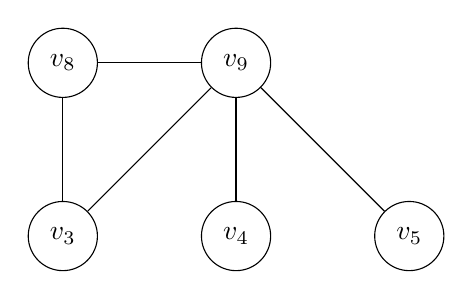
\begin{tikzpicture}[->, >=Stealth, auto, node distance=2.2cm]
			\node[state] (v8) {$v_8$};
			\node[state] (v9) [right of=v8] {$v_9$};
			\node[state] (v3) [below of=v8] {$v_3$};
			\node[state] (v4) [below of=v9] {$v_4$};
			\node[state] (v5) [right of=v4] {$v_5$};

			\path
			(v8) edge[-] (v9)
			(v8) edge[-] (v3)
			(v9) edge[-] (v3)
			(v9) edge[-] (v4)
			(v9) edge[-] (v5);
		\end{tikzpicture}
	\end{center}
	Instance 2:
	\[
	V=\set{v_1,v_2,v_3,v_4}, \quad E=\set{\set{v_1,v_2},\set{v_2,v_3},\set{v_1,v_4}}, \quad K=1
	\]
	\textbf{Answer: }Instance 1 is a YES-instance, as one of the possible solutions is $\set{v_9,v_8}$. Instance 2 can be shown to be a NO instance by looking at each vertex and seeing if it covers all others. You can then see that there is no solution with $K=1$ to this instance.


	\subsection{Now pick one of the instances, apply the reduction and show that result is still a yes-instance or no-instance (depending on which one you picked).}

	\begin{align*}
		&f(I_1)=\langle\\
		&\hspace{0.2cm} U=\set{v_3,v_4,v_5,v_8,v_9},\\
		&\hspace{0.2cm} C=\set{(v_3\vee v_8),(v_3\vee v_9),(v_8\vee v_9),(v_9\vee v_4),(v_9\vee v_5), (\neg v_3), (\neg v_4), (\neg v_5), (\neg v_8), (\neg v_9)},\\
		&\hspace{0.2cm} K=2 \\
		&\rangle
	\end{align*}
	Now take the assignment:
	$$\set{v_3=0,v_4=0,v_5=0,v_8=1,v_9=1}$$
	All clauses in $C$ are satisfied except for 2: $(\neg v_8)$ and $(\neg v_9)$. Therefore, this is a YES-instance of SatExcept.


	\subsection{Show that the reduction can be performed in polynomial time.}

	Stage 1 and 3 are obviously linear, as they just copy parts of the input to the output. Stage 2 first iterates over all edges and copies them over as clauses, which is linear in the number of edges, and then creates a clause for every node, which is obviously linear in the number of nodes. So overall stage 2 is in $O(n+m)$ which is still polynomial in the size of the overall input.

	\section{Exercise 6}
	Revision, old exam question midterm 20--21: Consider an NFA $N$ on the left and an NFA $N'$ on the right with transition diagrams as follows.

	\begin{center}
		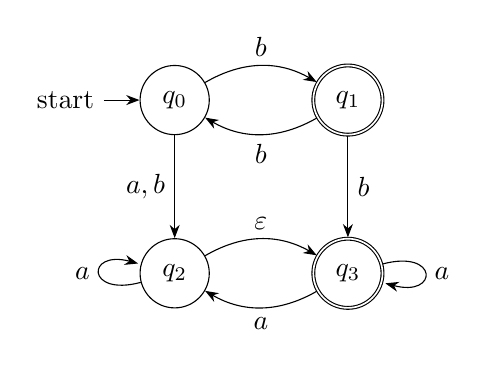
\begin{tikzpicture}[->, >=Stealth, auto, node distance=2.2cm]
			\node[initial,state] (q0) {$q_0$};
			\node[state,accepting] (q1) [right of=q0] {$q_1$};
			\node[state] (q2) [below of=q0] {$q_2$};
			\node[state,accepting] (q3) [right of=q2] {$q_3$};

			\path
			(q0) edge[bend left] node {$b$} (q1)
			(q1) edge[bend left] node {$b$} (q0)
			(q0) edge node[left] {$a,b$} (q2)
			(q1) edge node[right] {$b$} (q3)
			(q2) edge[loop left] node {$a$} (q2)
			(q2) edge[bend left] node {$\eps$} (q3)
			(q3) edge[bend left] node {$a$} (q2)
			(q3) edge[loop right] node {$a$} (q3);
		\end{tikzpicture}
		\hspace{1cm}
		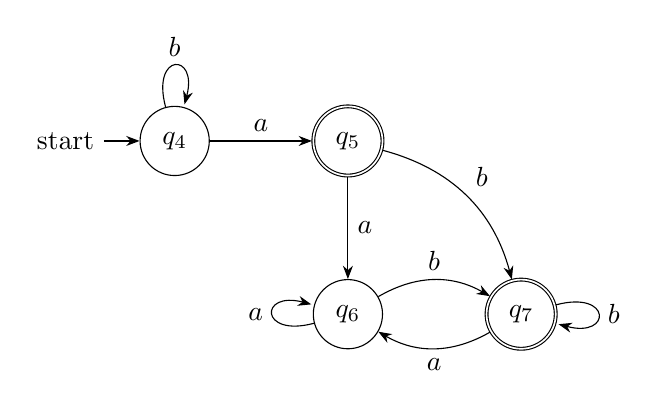
\begin{tikzpicture}[->, >=Stealth, auto, node distance=2.2cm]
			\node[initial,state] (q4) {$q_4$};
			\node[state,accepting] (q5) [right of=q4] {$q_5$};
			\node[state] (q6) [below of=q5] {$q_6$};
			\node[state,accepting] (q7) [right of=q6] {$q_7$};

			\path
			(q4) edge[loop above] node {$b$} (q4)
			(q4) edge node {$a$} (q5)
			(q5) edge node {$a$} (q6)
			(q5) edge[bend left] node {$b$} (q7)
			(q6) edge[loop left] node {$a$} (q6)
			(q6) edge[bend left] node {$b$} (q7)
			(q7) edge[bend left] node {$a$} (q6)
			(q7) edge[loop right] node {$b$} (q7);
		\end{tikzpicture}
	\end{center}

	Describe how you could use $N$ and $N'$ to construct an NFA $N''$ such that
	\[
	L(N'') = L(N)^* \circ L(N').
	\]
	(note the `star' symbol after $L(N)$). How would you combine them and what you would need to change? Make sure to explain it for this particular example rather than the general principle.

	\textbf{Answer: }To construct $L(N)^*$ You would start by adding a new accepting and initial state. You would add an $\eps$-transition from this new initial state to the old initial state and also add $\eps$-transitions from every accepting state to the old initial state. Lets call this new NFA $N_*$. Then, to create the concatenation between $L(N_*)$ and $L(N')$, we add $\eps$-transitions from every accepting state of $N_*$ ($q_1$ and $q_3$) to the initial state of $N'$ ($q_4$) and also remove the 'accepting' feature of $q_1$ and $q_3$ and remove the 'initial' feature of state $q_4$.

	\section{Exercise 7}
	Revision, old exam question endterm 21--22: For each of the following claims, show the claim is true or give a counterexample and explanation to show the claim is false, starting your answer with either ``True'' or ``False''.

	\subsection{If there is a direct reduction from $L$ to $A_{TM}$ and from $A_{TM}$ to $L$, then $\overline{L}$ is not Turing-recognisable.}

	\textbf{True. }$A_{TM}\leq_{TM}L\iff \overline{A_{TM}}\leq_{TM}\overline{L}$. So therefore, in $\overline{L}$ where Turing recognizable, then so would $\overline{A_{TM}}$ be, which we know it isn't.

	\subsection{If there is a Karp reduction $SAT \leq_P L$, then $L$ is undecidable.}

	\textbf{False. } We know $SAT$ to be NP Complete. And any $NPC$ problem is Karp reducible to any other $NPC$ problem. So take $L$ being any other NPC problem as a counterexample.

\end{document}